% !Mode:: "TeX:UTF-8"

%要运行该模板,LaTex需要安装CJK库以支持汉字.
%字体大小为12像素,文档类型为article
%如果你要写论文,就用report代替article
%所有LaTex文档开头必须使用这句话
\documentclass[12pt,twocolumn]{article}

%使用支持汉字的CJK包
\usepackage{CJKutf8}
\usepackage{indentfirst}
\usepackage[top=0.5in, bottom=0.5in, left=0.4in, right=0.4in]{geometry}
\usepackage[square,comma,numbers,sort&compress]{natbib}
\usepackage{graphicx}
\usepackage{booktabs}
\usepackage{tabularx}
\usepackage{enumitem}
\usepackage{titling}

\setlength{\parindent}{2em}
\setlength{\parskip}{0.5em}

\renewcommand{\contentsname}{目录}
\renewcommand{\listfigurename}{插图目录}
\renewcommand{\listtablename}{表格目录}
\renewcommand{\refname}{参考文献}
\renewcommand{\abstractname}{摘要}
\renewcommand{\indexname}{索引}
\renewcommand{\tablename}{表}
\renewcommand{\figurename}{图}

\setlength{\abovecaptionskip}{0em plus 0.3em minus 0.3em}
\setlength{\belowcaptionskip}{0em plus 0.3em minus 0.3em}
\setlength{\tabcolsep}{0.5em}
\setlength{\columnsep}{0.4in}

\linespread{1.1}

\setlist[1]{itemsep=0em,topsep=0em}

\renewcommand{\arraystretch}{1.3}

% make title left
\makeatletter
\renewcommand{\maketitle}{\bgroup\setlength{\parindent}{0pt}
\begin{flushleft}
  \LARGE {\textbf{\@title}}\vspace{1em}

  \normalsize{\@author}
\end{flushleft}\egroup
}
\makeatother

% change margin
\def\changemargin#1#2{\list{}{\rightmargin#2\leftmargin#1}\item[]}
\let\endchangemargin=\endlist

%开始CJK环境,只有在这句话之后,你才能使用汉字
%另外,如果在Linux下,请将文件的编码格式设置成GBK
%否则会显示乱码
\begin{CJK*}{UTF8}{gbsn}
\CJKindent
\CJKtilde

%这是文章的时间
%如果没有这行将显示当前时间
%如果不想显示时间则使用 \date{}
\date{}

%以上部分叫做"导言区",下面才开始写正文
\begin{document}

\twocolumn[
  \begin{@twocolumnfalse}
    %这是文章的标题
    \title{平行坐标综述}
    %这是文章的作者
    \author{赖楚凡\hspace{1em}袁晓如}
    %先插入标题
    \maketitle
    %\vspace{-4em}

    \begin{changemargin}{0.2in}{0in}
    {\bf 摘\hspace{1em}要:}
    \vspace{1em}

    {\bf 关键词:}
    \vspace{1em}
    \end{changemargin}

    %这是文章的标题
    \title{Parallel Coordinates}
    %这是文章的作者
    \author{Chufan Lai\hspace{1em}Xiaoru Yuan}
    %先插入标题
    \maketitle
    %\vspace{-4em}

    \begin{changemargin}{0.2in}{0in}
    {\bf Abstract: } 
    \vspace{1em}

    {\bf Keywords: }
    \vspace{2em}
    \end{changemargin}
  \end{@twocolumnfalse}
]

%再插入目录
%\tableofcontents
\section{引言}
\label{section:introduction}

在现实世界中,同一事物往往有多个不同的属性,要完整地描述该事物,需要记录其各个属性的信息。而这类具有多属性(维度)信息的数据,就称为多变量数据(Multivariate Data),或称高维数据(High-dimensional Data)。在传统的数据分析中,高维数据一般利用统计方法加以处理,并通过表格的方式呈现。但传统方法过于依赖自动算法,既无法结合用户的知识与判断,也不利于对抽象的高维信息的认知和理解。而信息可视化技术(Information Visualization)通过对高维数据的视觉呈现,辅以交互式的数据处理手段,能使用户充分参与到数据处理过程中,既加深了用户对数据的理解,也提高了数据分析的效率和可靠性。

高维数据一直是信息可视化领域的研究重点之一,其独有的两个特性:即维度数高、抽象性强,为可视化设计带来了巨大挑战。一方面,维度数的增长使得数据的信息量急剧增大,有限的显示空间只能表达一部分数据特征,而自动算法也会因为所谓的“维数灾难”(过高的复杂度、过低的采样率等\citep{Bellman1962})而难以应用。另一方面,由于人无法感知高于三维的拓扑空间,高维的数据特征(如聚类、流型等)往往抽象而难以理解。针对这些挑战,领域内提出了各类高维可视化方法\cite{grinstein2001high},包括降维投影\cite{fodor2002survey}、散点图矩阵\cite{cleveland1988dynamic}、雷达图\cite{hoffman1999dimensional}、星型坐标\cite{kandogan2000star}等等。而由Inselberg等人提出的平行坐标\cite{inselberg1985plane}也因其简单直观、可拓展性强等优点而被广泛应用于高维数据的可视分析中。

本文对

就具体设计而言,平行坐标的构造原理十分简单。
\begin{figure}[!htb]
\centering
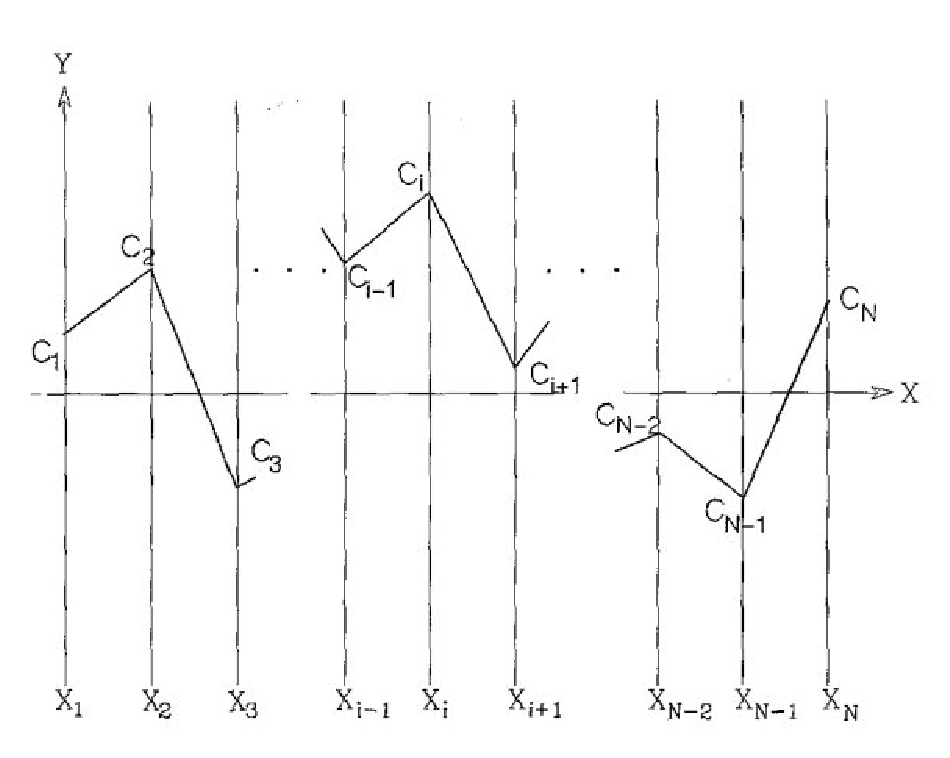
\includegraphics[width=1.0\linewidth]{images/PC_principle.eps}
\caption{\label{fig:overview_method}轨迹数据可视分析的三种方法。本图修改自Andrienko~等人的论文~\citep{AndrienkoADFW2008}~。
}
\end{figure}

\section{基本原理}
\label{section:basics}


\section{平行坐标的改进}
\label{section:improvements}

\section{平行坐标的应用}
\label{section:applications}

\section{问题与挑战}
\label{section:challenges}

\section{结论}
\label{section:conclusion}

\bibliographystyle{abbrvnat}
%\setcitestyle{aysep={,},yysep={;}}
\bibliography{parallelcoordinates}
	
\end{CJK*}
\end{document}

